\chapter{进一步工作}

\section{缺陷}

本文在此前的篇幅已经叙述过与 watchOS 、 LeapMotion 这些相关硬件开发上不可逾越的困难,在性能和功耗都严重受到限制 watchOS 上,交互消息的通信和处理都非常关键,一个良好的设计能够让各部分硬件顺利工作。然而软件是依赖硬件设计而成,因此接下来我们考虑在硬件实现本身和择备交互方案本身存在的问题。

\subsection{硬件缺陷}

作为一个原型项目,本文实现上使用 LeapMotion 完成对手部的的建模和识别,但 LeapMotion 自身却又限制在必须与一个桌面端系统进行连接,这就极大的限制了交互的范围和场景,不能在其他场景下使用。

在文\cite{Bailly:2012:SNP:2207676.2208576}中,Gilles 等人将一颗深度摄像头绑定在鞋子顶部,并在用户和腰部设置一个处理硬件用于识别交互,从而在鞋子顶部的上方制造了交互区域。类似的,我们可以设计图\ref{fig:hardware}所示的一个可移动的 LeapMotion 识别方案。

\begin{figure}[H]
    \kaishu
    \centering
    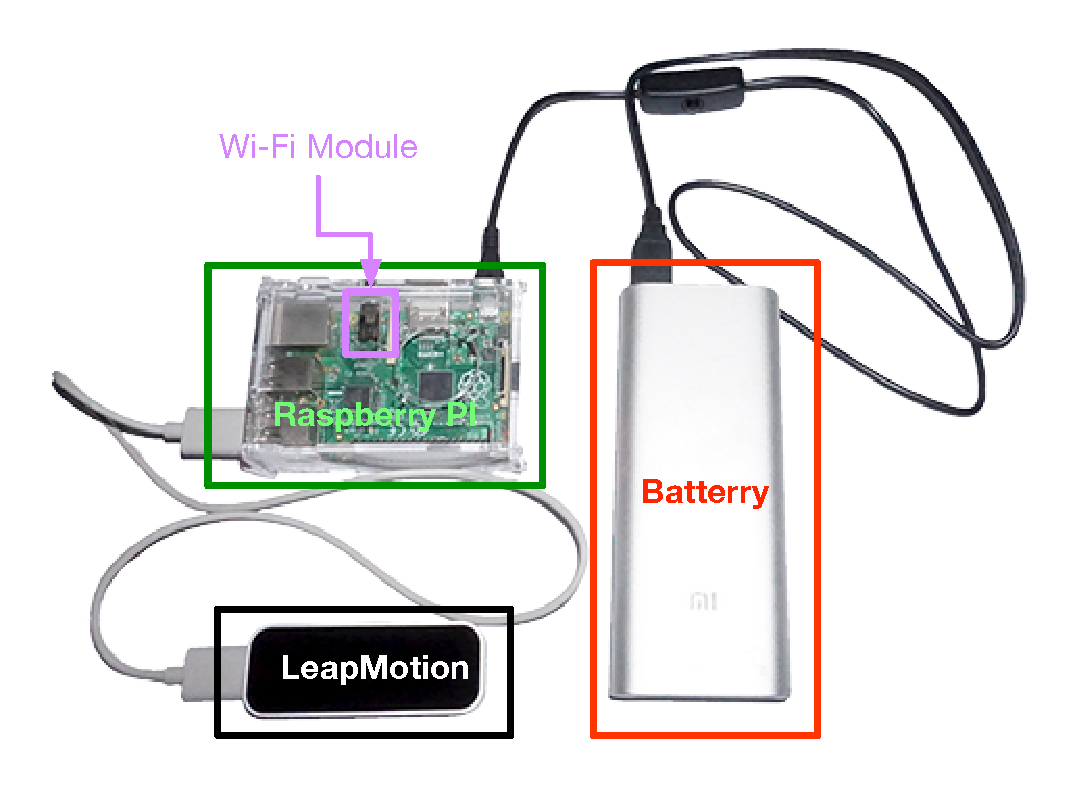
\includegraphics[width=0.6\textwidth]{figures/hardware}
    \caption{\kaishu \textbf{硬件结构}: 图中由三部分硬件分别为一个 5V-2A 输出功率的移动电源、一个组装了 WiFi 模组的树莓派 B+、一个 LeapMotion 硬件}
    \label{fig:hardware}
\end{figure}

在这个方案中,移动电源提供5V-2A 的输出功率,驱动树莓派;树莓派通过 WiFi 模组进而连接服务器进行交互信息通信,而 LeapMotion 则通过 USB 连接到树莓派上,只要树莓派上能够使用 LeapMotion 的软件部分,则此方案能够解决交互范围受限的问题。

遗憾的是,LeapMotion 软件要求宿主 OS 至少具备 2GB RAM,且 SDK 也仅能在 Ubuntu Linux 上得到支持,当前的树莓派第二代 B+仅有 512MB RAM,暂时得到应用,但随着 Windows 10能够在树莓派第三代上运行,我们有望看到未来当树莓派扩展到2GB RAM 时能够搭载 Windows 平台将图 \ref{fig:hardware} 的方案得到应用。

\subsection{交互缺陷}

本文给出的备择设计虽然从交互形式的表面上完整对接了原有的设计,但是一旦用户任务复杂时,此备择设计的效率则会劣于接触式设计。受到 Keystroke-Level Model (KL 模型)\cite{Card:1980:KMU:358886.358895}的启发,我们可以给出手表任务上的 KL 模型,并将一个用户任务分解为几个基础步骤,见表\ref{table:task}:

\begin{table}[H]
    %\scriptsize
    \small
    \kaishu
    \centering
    \begin{tabular}{c l}
        \toprule
        \textbf{变量}        & \textbf{描述} \\
        \hline
        $K$     & 普通点按操作 \\
        $F$     & Force Touch 操作 \\
        $S$     & 滑动操作 \\
        $T$     & 交互目标选定 \\
        $R$     & 系统响应 \\
        $M$     & 用户思考 \\
        $H$     & 最高优先级操作 \\
        \bottomrule
    \end{tabular}
    \caption{用户任务基础步骤}
    \label{table:task}
\end{table}

对普通点按而言,我们不妨假设双指捏合与屏幕点按的用时一致,注意到在备择设计中,目标的点按还需要通过双指滑动操作在屏幕上进行选取,故$K_{\text{contact-free}}>K_{\text{contact}}$;对 Force Touch 而言,接触式交互能够直接测量用户的按压力度,故即便对于 Force Touch 依然能够在普通点按的时间内完成,我们也不妨假设这两个时间相等,在\ref{sub:force-touch-simu}一节中,我们给出的对 Force Touch 仿真的方法是设定触摸事件的两个阶段,在第一个阶段内将点按处理为普通点击事件,显然我们有$F_{\text{contact-free}}>F_{\text{contact}}$。

对于 $T$、$M$ 和 $H$ 而言,如果用户已经熟悉这两种设计,我们不妨认为在两种设计上的用时相等。而对于 $T$ 参数,背着设计需要一个一个将视图中的对象进行遍历,显然$T_{\text{contact-free}}>T_{\text{contact}}$。另外,备择设计需要在通信上有所开销,因此$R_{\text{contact-free}}>R_{\text{contact}}$。

最后,接触式交互和非接触式交互都只能是以上七个基础步骤的线性组合,而对于同一个任务来说,其系数相同,根据上面的分析,显然有式\ref{eq:task-time}成立:
\begin{equation}
    \label{eq:task-time}
    \Sigma_{K,F,S,T,R,M,H}{\text{Contact Task}} < \Sigma_{K,F,S,T,R,M,H}{\text{Contact-free Task}}
\end{equation}
并且当任务变得复杂时,式\ref{eq:task-time}左式的值会明显小于右式。

\section{改进方向}

最后,我们对本文所设计系统在未来应用时植入方式的改进,以及系统整体的扩展性进行初步探讨。

\subsection{识别方式}

本文在手部信息的检测上使用了 LeapMotion 硬件作为解决问题的关键,但实际上 LeapMotion 是一项作为桌面端交互或虚拟现实交互的输入设备而产生的,依赖视觉方法的 LeapMotion 并不完全适合作为用户的一个随身穿戴部件植入,因为视觉方法的依赖性很强。考虑手表本身的设计,我们可以考虑更换一种对手势进行识别的方式。

Myo \cite{Myo:2016} 是一个固定在手臂上的对手部肌肉电信号进行感知从而进行手势识别的装置,如图\ref{fig:myo}所示。Myo 通过内置的 Wi-Fi 装置将识别的电信号传递给其他的连接部件,Myo 开放了并规范化了对手部肌肉电信号时间序列的识别协议,这意味着我们可以对这种表现模式的手势数据进行分析,进而逐步完善手势系统。

\begin{figure}[H]
    \kaishu
    \centering
    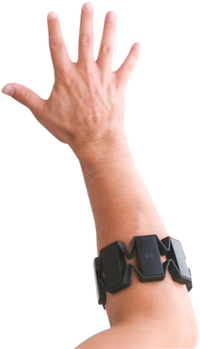
\includegraphics[width=0.15\textwidth]{figures/myo}
    \caption{\kaishu \textbf{Myo 识别装置}: Myo 安装在手臂上对手部肌肉的电信号进行检测,从而根据这些电信号在时间序列上的变化特征进行手势识别。}
    \label{fig:myo}
\end{figure}

Myo 的设计实际上完全符合手表的人体工程学设计,因为手表的表带就是 Myo 最好的存在形式。当 Myo 能够缩小并设计成手表的表带时,这时手表系统本身在识别上不再依赖其他额外的设备,大幅降低设备间通信的消耗,便更加高效的完成交互。

\subsection{交互感知中心}

在 \ref{sub:im-arch} 一节中,我们讨论了通信架构的设计,实际上这一设计也适用于一般情况。

图 \ref{fig:universe-arch} 为对前文中适用于手表备择设计的通信架构的推广设计,在服务端和客户端引入了交互感知中心(Interaction Perception Center, IPC 是一个基于桌面端和移动端设备的跨平台交互解决方案)服务\cite{Changkun:2015ipc}。当我们将 IPC 这系统级的交互模型引入时,实现 IPC 核心服务的传感器处理协议(Sensor Handle Protocol, SH协议)能够屏蔽掉硬件之间的差异,统一的将传感器形式化、标准化,而通过跨设备交互协议(Cross-Device Interaction Protocol, CDI协议)能实现用户设备与 IPC 服务之间的通信。

\begin{figure}[H]
    \kaishu
    \centering
    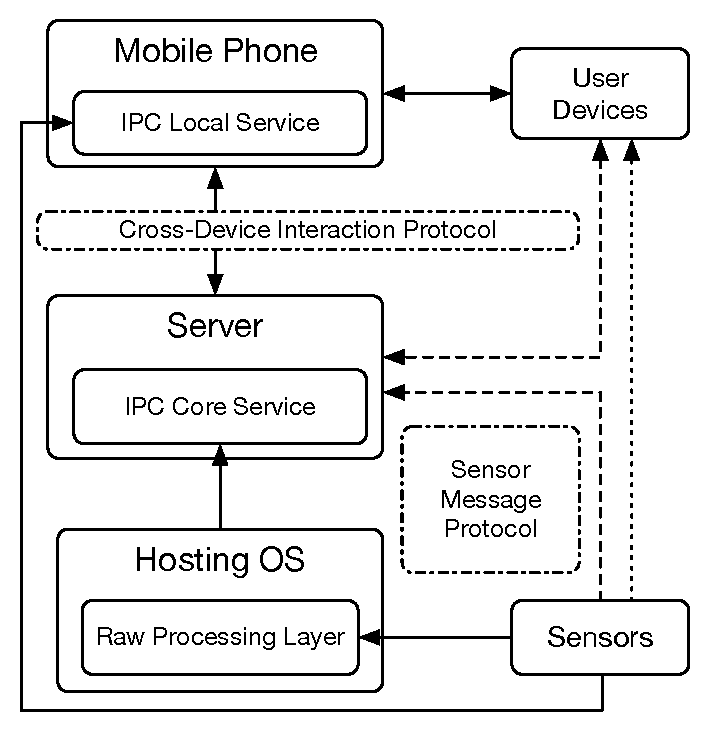
\includegraphics[width=0.4\textwidth]{figures/universe-arch}
    \caption{\kaishu \textbf{通用通信架构}: 在服务端和客户端引入了 IPC 服务。}
    \label{fig:universe-arch}
\end{figure}

不同的传感器先在与其连接的桌面端系统上按传感器各自的 SH 协议对原始数据进行初步加工,再由 OS 将这些消息集中发送给服务端交给 IPC 核心服务进行处理进行二次加工,完成后再由服务端请求层按 CDI 协议进行封装并分发给相应的设备;另一方面,当 IPC 核心服务不可用时,传感器的宿主 OS 依然能与客户端的本地 IPC 服务进行通信,使得在服务器离线状态下依然能够响应一些简单的交互。

IPC 设计之初是一个纯软件的解决方案,目的是解决桌面端设备和移动端设备的跨平台分布式数据通信与分析,而从前文中的基础通信架构设计中我们能够得到启示:首先,统一交互系统的设计不宜将传感器原始数据直接发送给 IPC 服务器进行分析,传感器的数据应当在传感器的宿主 OS 上完成对数据的基础加工,加工后的数据和 IPC 服务器之间增加一层消息协议来保证任何传感器数据都能接入 IPC 的接口;其次,IPC 传递给用户设备的交互消息需是用户可选的,这些交互在任何情况下,都至少有一种主交互方案。即被动交互应当是隐式、备择的。

\section{结束语}

本文对智能手表上现有的交互形式进行了备择设计,配合了 Haptic Engine 对用户的直观震动反馈,完成了对基础点按、滑动、Digital Crown、Force Touch等系列原生手势的备择设计,将十种原生交互简化为了八种备择交互,且消除了接触式交互的依赖,并说明了此套备择设计的交互完备性。与主流交互不同,备择交互更像是编程语言上的一个语法糖,其侧重于临时、快捷、简便的实现一个用户期望的输入。在本次的设计中,我们克服了从硬件平台到软件框架接口不支持缺陷,在克服这些缺陷中发展出来的架构设计给与了我们在整合一套交互系统时的很多有益启示。

总的来说,人机交互的创新往往伴随着硬件和软件的结合,在软件层的方法有时往往会受到硬件平台的各种限制,一套打通硬件与软件的架构设计不仅涉及从硬件到软件的垂直整合能力,还需要进行横向设计与可用性的考量,这些内容浮与水面之上,也仅仅只是冰山的一角。
